\documentclass{deliverablereport}
\usepackage{pdfpages}

\deliverable{dissem}{short-course}
\deliverydate{02/27/2017}
\duedate{02/27/2017 (Month 18)}
\def\pn{OpenDreamKit}
\author{Mike Croucher and Tania Allard}

\begin{document}
\maketitle
\strut\githubissuedescription
\tableofcontents\newpage
\section{Workshops}
The first stage of evolution of the course material was to develop and deliver an instructor-led workshop for lecturers at The University of Sheffield.
This workshop was delivered in June 2016 to approximately 20 lecturers, primarily from Sheffield's physics department. Feedback from the workshop informed future development and the workshop material became the nucleus of the current deliverable.
\section{Course Website}
We have produced a website, \url{https://mikecroucher.github.io/SMC_tutorial/}, containing a set of tutorials for educators who wish to adopt SageMathCloud in their teaching. The course material is developed in a style that allows it to be used for self-directed study as well as in instructor-led workshops.
Access logs indicate that the GitHub repository hosting the material is visited by at least 40 unique visitors a week. This is in addition to visitors to the website itself that we currently do not measure.

In order to facilitate sustainability of the project, the website is
developed on the open source collaboration platform \GitHub, using a standard and open set of web technologies (Markdown and Jekyll). As such, it is possible for anyone in the world to comment on, contribute to, and collaborate with the project.
Several individuals outside of the OpenDreamKit consortium have already made contributions.

The material has been adopted by the SageMathCloud development team and forms part of the official documentation.
\section{Implementation at University of Sheffield}
The University of Sheffield has been used as a testbed for both SageMathCloud and this tutorial material. Workshops have been delivered to educators from the departments of physics, biomedical sciences and computer science. In all cases, this resulted in the development and delivery of undergraduate and postgraduate courses using this technology stack. Highlights include 'Bioinformatics for Biomedical Sciences',which is currently being used by the University of Sheffield as a case study for 'excellence in teaching' (Appendix A and \url{https://www.sheffield.ac.uk/bms/teaching/stories/bms353}), and the departmental-wide adoption of SageMathCloud and Jupyter Notebook by the department of physics and astronomy who use it in several undergraduate courses spanning the entire curriculum.

Dr Mark Quinn, a University teacher from Sheffield, attended the 2017 OpenDreamKit dissemination workshop, Computational Mathematics with Jupyter (\url{http://opendreamkit.org/meetings/2017-01-16-ICMS/}). In his presentation (Appendix B and \url{http://opendreamkit.org/meetings/2017-01-16-ICMS/talks/SMC_Sheffield.pdf}), Mark notes that ALL current physics undergraduates (several hundred students) at Sheffield are now coding using SageMathCloud and that this process began with the workshop that eventually developed into the material that forms this deliverable.
\section{Future Work}
\begin{itemize}
\item Continue the collaboration with University Of Sheffield's physics department who is beginning to conduct research into the efficacy of Jupyter notebooks and SageMathCloud in teaching.
\item Use this material to work with other departments within The University of Sheffield to expand the reach of this technology stack. Potential future collaborators include the departments of Architecture, Mathematics, and Engineering.
\item Deliver workshops based on this material to Universities around Europe.
\end{itemize}

\appendix
\section{27 Feb 2017, BMS353 Case Study, University of Sheffield website}
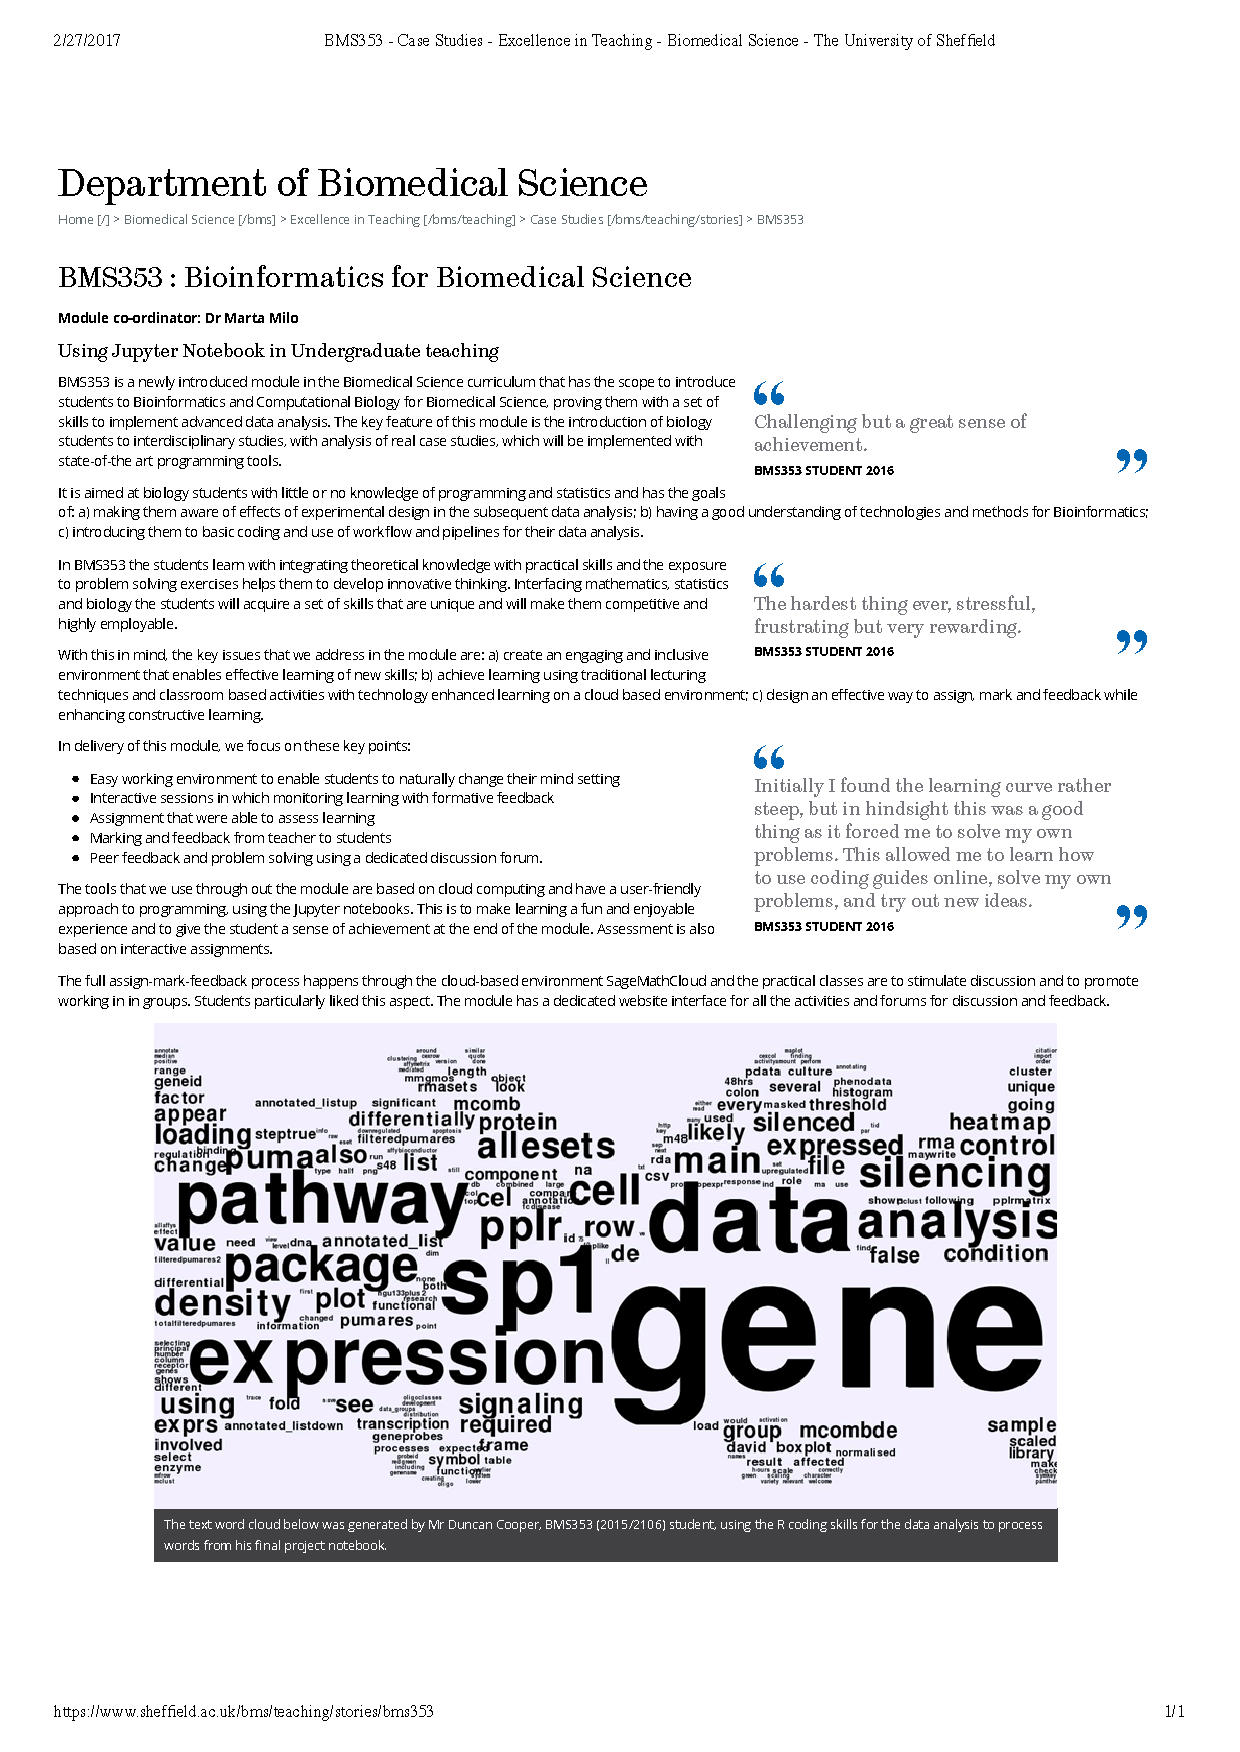
\includepdf{BMS353_CaseStudies.pdf}
\section{16 Jan 2017, Using SageMathCloud for teaching undergraduate physics, Presentation at OpenDreamKit dissemination workshop 'Computational Mathematics with Jupyter'}
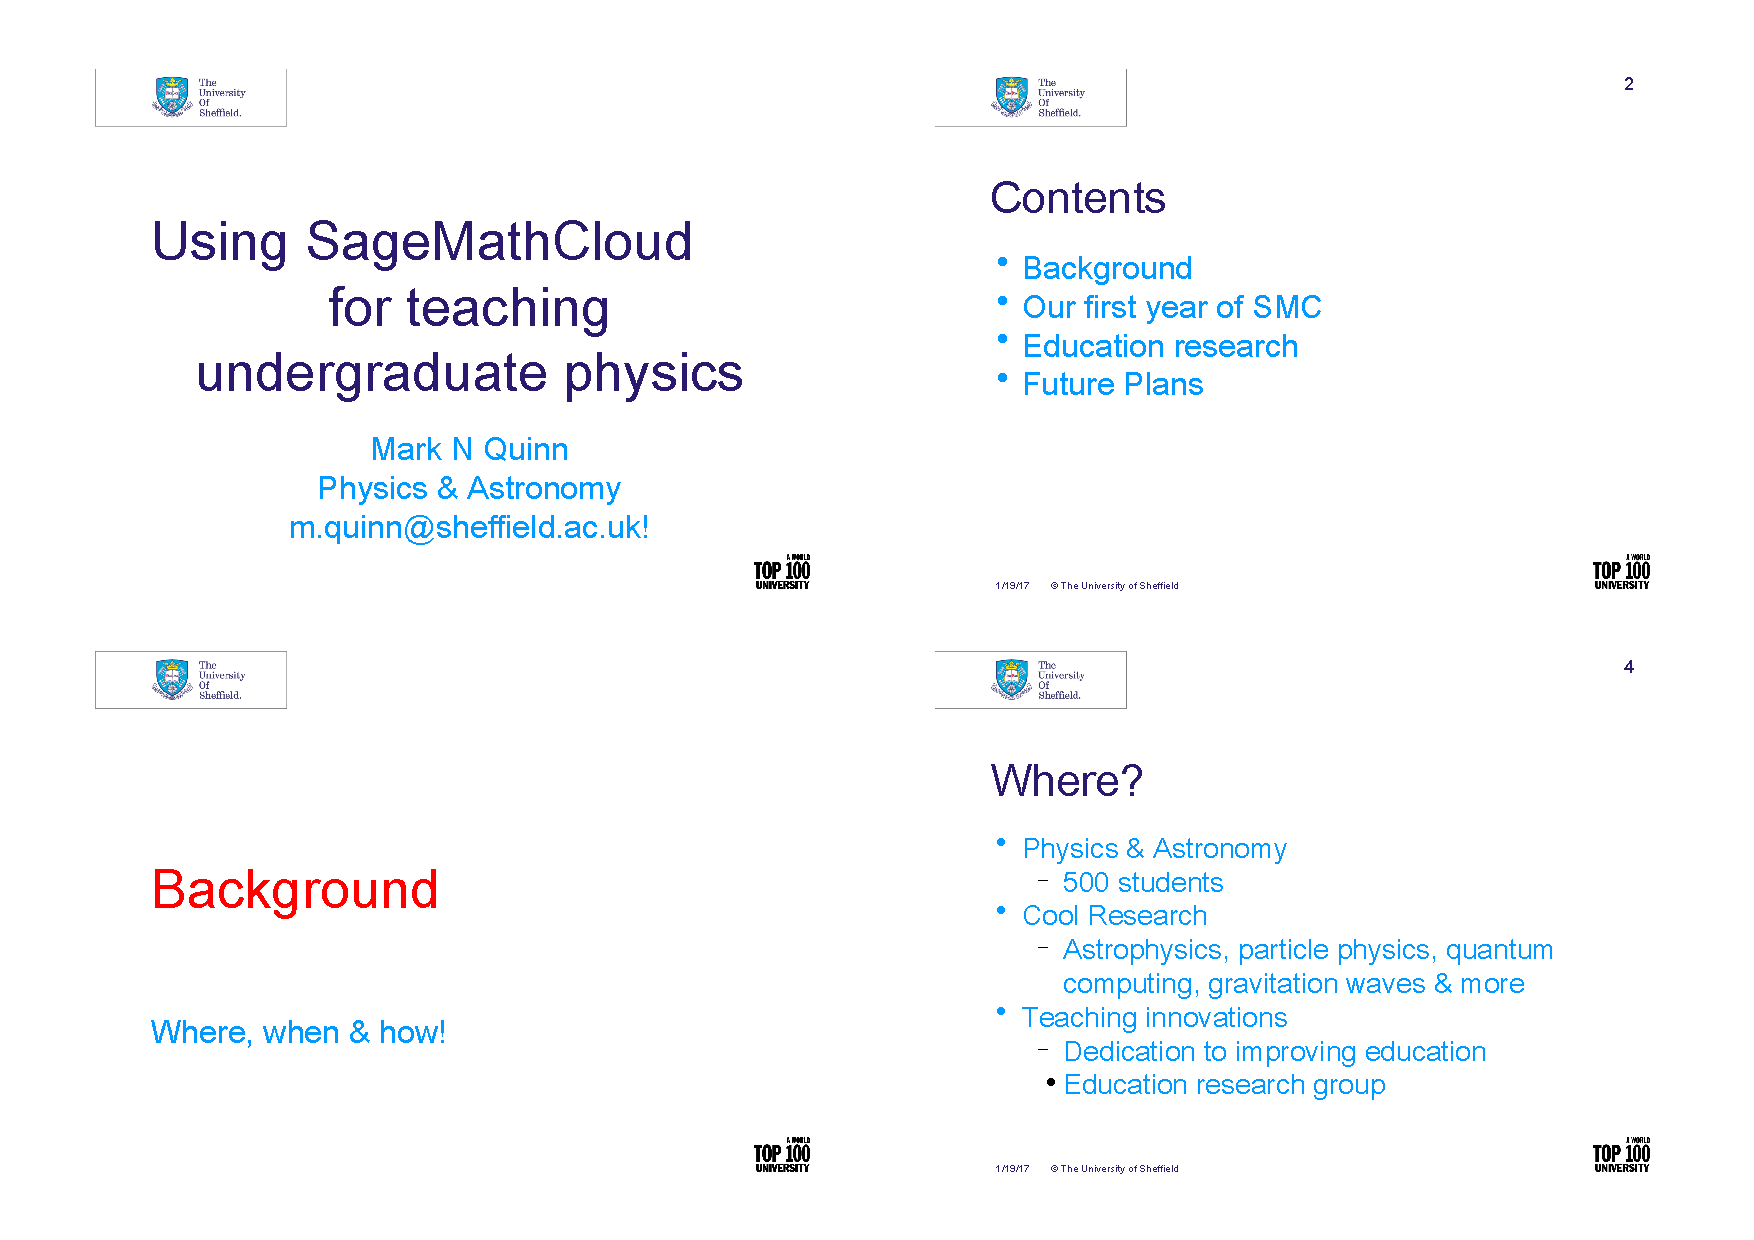
\includepdf[pages={1-9}]{SMC_Sheffield_4.pdf}

\end{document}

%%% Local Variables:
%%% mode: latex
%%% TeX-master: t
%%% End:

%  LocalWords:  githubissuedescription newpage tableofcontents newpage printbibliography
